\newpage
\appendix
\section{Discussion and Experimental Details}
\subsection{Discussion of Baseline Methods}
\label{appendix:baseline_detail}
In this paper, we mainly compare our method to baselines that attempt to improve MLE by optimizing distance measures beyond forward cross-entropy.
\paragraph{TaiLr} \cite{tailr} proposes to leverage the total variation distance~(TVD) as a more robust alternative to the forward cross-entropy for language generation model training. Specifically, they introduce a token-level factorization of the original TVD and optimize its upper bound in addition to the MLE loss. The training objective of TaiLr can be written as:
\begin{equation}
    \mathcal{L}_{\text{TaiLr}}=-\frac{Q_{\theta}(x_t|x_{<t})}{\gamma+(1-\gamma)Q_{\theta}(x_t|x_{<t})}\log{Q_{\theta}(x_t|x_{<t})}
    \label{eq:tailr}
\end{equation}
From the form of Eq.~\ref{eq:tailr} we can see that TaiLR only alleviates the recall-prioritization issue of MLE while still confronting the negative diversity ignorance and train-test mismatch problems.
\paragraph{MixCE} \cite{mixce} is another modification to MLE which incorporates the reverse cross-entropy into the training objective. Due to the one-hot encoded token-level data distribution, the author proposes an approximation and uses an interpolation coefficient to combine it with forward cross-entropy as follows:
\begin{equation}
    \mathcal{L}_{\text{mixce}}=-(\gamma+(1-\gamma)Q_{\theta}(x_t|x_{<t}))\log{Q_{\theta}(x_t|x_{<t})}
    \label{eq:mixce}
\end{equation}
Both Eq.~\ref{eq:tailr} and Eq.~\ref{eq:mixce} can be regarded as the original $\mathcal{L}_{\text{MLE}}$ multiplied by a coefficient determined by a tunable hyper-parameter $\gamma$ and model's probability~(confidence) of $x_t$. Though attractive in terms of their original formulation, TaiLr and MixCE both degenerate into certain regularized forms of MLE, hence demonstrating limited improvements.
\subsection{Differences between EMO and Reinforcement Learning from Human Feedback~(RLHF)}
\label{appendix:rlhf}
Prevailing methodologies impart the desired behaviors into a base language model through meticulously crafted human preferences that represent the types of responses that humans find helpful. This stage, dubbed supervised fine-tuning~(SFT), often happens after the initial unsupervised pre-training on a large text dataset. 
Although the STF models already exhibit good instruction-following capabilities, the common practice is to further align their behavior with human value, a procedure known as Reinforcement Learning from Human Feedback~(RLHF)~\citep{christiano2017deep,ziegler2019fine,bai2022constitutional}. 

The differences between EMO and RLHF manifest in multiple dimensions, including motivation, gradient, and application scenario. In the following, we discuss these points in detail.
\begin{itemize}
    \item \textbf{Motivation}: The motivation behind EMO is to explore effective means to adapt a language model to a given human text dataset through the lens of earth-mover distance optimization. Evaluation is thus focused on quantifying how similar the model distribution $Q_{\theta}(\bm{x})$ is to human text distribution $P(\bm{x})$. In contrast, RLHF prioritizes steering the behavior of the language model based on the feedback provided by a specific reward model~(PPO~\citep{ppo}) or directly from existing human preference dataset~(DPO~\citep{dpo}). The evaluation is often based on human-centric subjective metrics such as helpfulness and safety. 
    \item \textbf{Gradient}: The per time step gradient of EMO is the combination of gradient of probability of \textbf{each token in the vocabulary}, weighted by their respective expected transport costs, i.e., $\sum_{i=1}^{|V|}\nabla_{\theta}Q_{\theta}(v_i)\mathbb{E}_{v_j\sim P}[C(v_i,v_j)]$. For PPO, the per time step gradient is the gradient of \textbf{current token}'s log probability, weighted by the reward $r(\bm{x},\bm{y})$ and the deviation from a reference model $D_{KL}(Q_{\theta}(\bm{y}|\bm{x})||Q_{\text{ref}}(\bm{y}|\bm{x}))$, i.e., $\nabla_{\theta}\log{Q_{\theta}(y_t|\bm{x},\bm{y}_{<t})}(r(\bm{x},\bm{y})-\log{\frac{Q_{\theta}(y_t)}{Q_{\text{ref}}(y_t)}})$. For DPO, the per time step gradient is the gradient of the \textbf{current token}(in the preferred or dispreferred response)'s log probability, weighted by the incorrectness value of an implicit reward model, i.e., $\nabla_{\theta}\log{Q_{\theta}(y_t|\bm{x},\bm{y}_{<t})}\cdot \sigmoid(\beta\log{\frac{Q_{\theta}(y_l)}{Q_{\text{ref}}(y_l)}}-\beta\log{\frac{Q_{\theta}(y_w)}{Q_{\text{ref}}(y_w)}})$.
    \item \textbf{Application Scenario}: As a general-purpose objective for auto-regressive language modeling, EMO is applicable to domain-specific fine-tuning/adaptation, instruction-tuning, and continual pre-training. Currently, the use of RLHF predominantly occurs in the alignment stage after supervised fine-tuning.
\end{itemize}


\subsection{Dynamic Weighting}
\label{appendix:dynamic}
In situations where the language model is relatively weak~(having high perplexity), DEMD may converge at a slow pace due to bounded gradient scaling induced by cosine-based transport cost. To overcome this potential issue, the final loss function in EMO is implemented as a dynamically weighted combination of MLE and DEMD:
\begin{align}
    \mathcal{L}=0.5*(\mathcal{L}_{\text{MLE}} + (\frac{\mathcal{L}_{\text{MLE}}}{\mathcal{L}_{\text{DEMD}}}).\text{detach()}*\mathcal{L}_{\text{DEMD}})
\end{align}
\subsection{Open-ended Generation}
\label{appendix:a1}
\begin{table}[h!]
    \centering
    \scriptsize
    \begin{tabular}{ccccccc}
    \toprule
    \textbf{Datasets} & \textbf{WikiText2} & \textbf{Wikitext103} & \textbf{WebText} & \textbf{PTB} & \textbf{WritingPrompts} & \textbf{AG News} \\
    \midrule
    \# of train samples     &36,700                   & 1,800,000             & 20,000              &4,210            &10,000                 &112,000                \\
    \# of dev samples     & 3,760                  &  3,760                   & 5,000               &3,370            &925                       &6,000               \\
    \# of test samples     & 4,360                  & 4.360                    &5,000                &3,760           &1,047                       &7,600                \\
    \midrule
    prefix length     & 20                  & 20                    & 20               & 5            & 35                      & 10               \\
    generation length & 80                  & 80                    & 80               & 25           & 80                      & 30               \\
    \bottomrule
    \end{tabular}
    \caption{Length of the provided prefix and model generations for each dataset employed in the open-ended generation experiments.}
    \label{table:stat}
\end{table}
We provide the detailed statistics and settings in the open-ended generation experiment in Table.~\ref{table:stat}. For WikiText2, Wikitext103, PTB, and AG News, we download the datasets from the HuggingFace Datasets hub. For WritingPrompts and WebText, we utilize the official split provided by \cite{mixce}.

\subsubsection{Quantifying the Precision-Recall Tradeoff}
\label{appendix:p_r}
To have a quantitative understanding of how MLE is biased towards recall, we visualize the averaged token-level forward and reverse cross-entropy between $Q_{\theta}$ of a GPT-2 model fine-tuned with different objectives and that of a pre-trained GPT-Neo-1.3B~\citep{gpt-neo} model~(which serves as a surrogate target distribution) in Fig.~\ref{fig:p_r}. TaiLr and MixCE demonstrate an improved balance between precision and recall, while our proposed EMO further outperforms these two methods with significant margins.
\begin{figure}[h]
    \centering
    \scalebox{0.965}{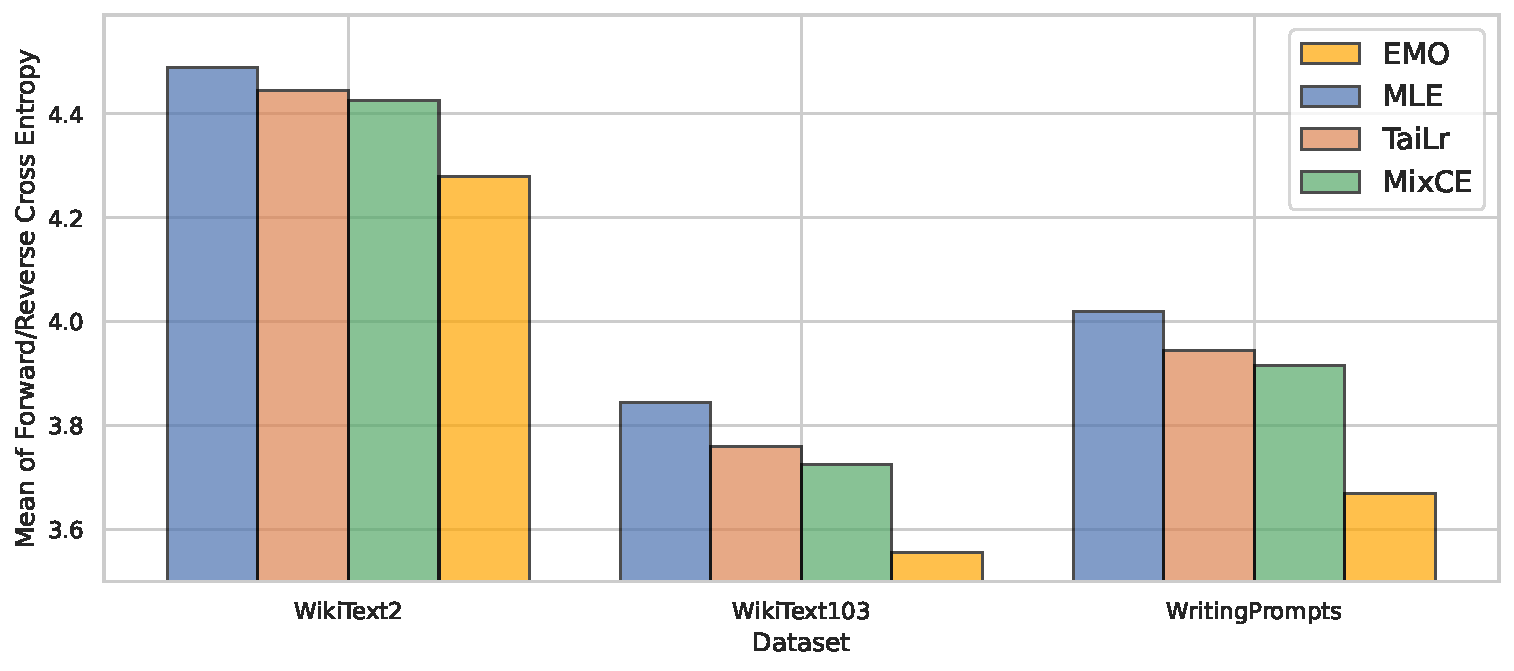
\includegraphics[width=0.99\textwidth]{./figures/mean_p_r.pdf}}
    \caption{The average of token-level forward and reverse cross-entropy between distribution $Q_{\theta}$ of GPT-2 fine-tuned with different objectives and that of GPT-Neo-1.3B on the validation set of three different datasets. The lower the value, the better the learned $Q_{\theta}$ balance precision and recall.}
    \label{fig:p_r}
\end{figure}

\subsection{Prompt Templates for Language Understanding Tasks}
\label{appendix:a2}
% Please add the following required packages to your document preamble:
% \usepackage{multirow}
\begin{table}[h]
    \centering
    \scriptsize
    \begin{tabular}{ccc}
    \toprule
    \textbf{Tasks}                            & \textbf{Prompts}                                                                              & \textbf{Label}                            \\
    \midrule
    \multirow{2}{*}{SST-2}           & Review: ``\textless{}X\textgreater{}'' It is positive.                                 & Positive                         \\
                                     & Review: ``\textless{}X\textgreater{}'' It is negative.                                 & Negative                         \\
    \midrule
    \multirow{4}{*}{Tweet Emotion}   & Tweet: ``\textless{}X\textgreater{}'' It is anger.                                     & Anger                            \\
                                     & Tweet: ``textless{}X\textgreater{}'' It is joy.                                       & Joy                              \\
                                     & Tweet: ``\textless{}X\textgreater{}'' It is optimism.                                  & Optimism                         \\
                                     & Tweet: ``\textless{}X\textgreater{}'' It is sadness.                                   & Sadness                          \\
    \midrule
    \multirow{6}{*}{TREC}            & Question: ``\textless{}X\textgreater{}'' It is about abbreviation.                     & Abbreviation                     \\
                                     & Question: ``\textless{}X\textgreater{}'' It is about entity.                           & Entity                           \\
                                     & Question: ``\textless{}X\textgreater{}'' It is about description and abstract concept. & Description and abstract concept \\
                                     & Question: ``\textless{}X\textgreater{}'' It is about human being.                      & Human being                      \\
                                     & Question: ``\textless{}X\textgreater{}'' It is about location.                         & Location                         \\
                                     & Question: ``\textless{}X\textgreater{}'' It is about numerical value.                  & Numerical value                  \\
    \midrule
    \multirow{2}{*}{Subj}            & ``\textless{}X\textgreater{}'' It is objective.                                        & Objective                        \\
                                     & ``\textless{}X\textgreater{}'' It is subjective.                                       & Subjective                       \\
    \midrule
    \multirow{2}{*}{CR}              & Review: ``\textless{}X\textgreater{}'' It is positive.                                 & Positive                         \\
                                     & Review: ``\textless{}X\textgreater{}'' It is negative.                                 & Negative                         \\
    \midrule
    \multirow{2}{*}{Rotten Tomatoes} & Review: ``\textless{}X\textgreater{}'' It is positive.                                 & Positive                         \\
                                     & Review: ``\textless{}X\textgreater{}'' It is negative.                                 & Negative                         \\
    \midrule
    \multirow{4}{*}{AG News}         & ``\textless{}X\textgreater{}'' It is about world.                                      & World                            \\
                                     & ``\textless{}X\textgreater{}'' It is about sports.                                     & Sport                            \\
                                     & ``\textless{}X\textgreater{}'' It is about business.                                   & Business                         \\
                                     & ``\textless{}X\textgreater{}'' It is about science and technology.                     & Science and Technology          \\
    \bottomrule                                    
    \end{tabular}
    \caption{Prompt templates for natural language understanding tasks used in Sec~.\ref{sec:nlu}. \textless{}X\textgreater{} is a placeholder that indicates the real input context/question.}
    \label{table:prompt}
\end{table}
The specific prompt templates used for each task in Sec.~\ref{sec:nlu} are presented in Table.\ref{table:prompt}. For MMLU, we follow the prompt design in \cite{2023opencompass}~\footnote{\url{https://github.com/open-compass/opencompass.}}. In implementation, each test input is prepended with 8 demonstrations that are retrieved using a pre-trained dense retriever based on semantic similarity. One exception is MMLU, where we adopt a fixed 5-shot demonstration following previous works. We compute the perplexity for the constructed prompt corresponding to each 
candidate answer and choose the one with the smallest perplexity as the final prediction.
Evaluations are implemented based on the OpenICL~\citep{wu-etal-2023-openicl} library.

\section{Additional Results on Language Understanding}
\label{appendix:a3}
\begin{table}[h!]
    \centering
    \small
    \begin{tabular}{ccccccccc}
    \toprule
    \textbf{Methods} & \textbf{TE} & \textbf{SST-2} & \textbf{TREC} & \textbf{Subj} & \textbf{CR}   & \textbf{RT} & \textbf{AG} & \textbf{MMLU} \\
    \midrule
    Pre-trained      &  56.7                   &95.4            &74.6           &76.2           &\textbf{93.6}           & 91.6                     & 86.2              & 43.6          \\
    MLE              & 58.4                    & 95.8           &72.4           & 74.6          & 93.4          &  92.1                    &  86.0             & 43.3          \\
    TaiLr            &  62.4                  & 95.9          & 74.6          &  81.0         &92.8           &  92.5                    & 87.4              &44.4           \\
    MixCE            &  66.5                   & \textbf{95.9}           & 77.6          &82.5  &93.1           & 92.1                     &  88.0            &  45.1         \\
    \midrule
    EMO             & \textbf{69.0}           &95.8   &\textbf{78.0}  &\textbf{83.1}           &93.4  &\textbf{92.8}                      &\textbf{88.1}      & \textbf{45.5}          \\
    \bottomrule
    \end{tabular}
    \caption{Downstream task performance of LLaMa2-7B fine-tuned with different training objectives on WikiText-103.}
    \label{table:llama2-7b}
\end{table}
\begin{table}[h!]
    \centering
    \small
    \begin{tabular}{ccccccccc}
    \toprule
    \textbf{Methods} & \textbf{TE} & \textbf{SST-2} & \textbf{TREC} & \textbf{Subj} & \textbf{CR}   & \textbf{RT} & \textbf{AG} & \textbf{MMLU} \\
    \midrule
    Pre-trained      &60.4                     &95.5            &80.4           &81.7           &91.2           &90.1                      &86.5               &54.7           \\
    MLE              &60.9                     &95.8            &81.0           &81.8           &90.9           &89.6                      &86.2               &54.3           \\
    TaiLr            &61.7                    &96.2           &80.4           &81.4           &\textbf{91.5}           &90.5                      &87.2               &54.5           \\
    MixCE            &64.4                     &95.7            &83.6           &84.7  &91.2           &90.4                      &87.4              &55.0           \\
    \midrule
    EMO             &\textbf{70.7}            &\textbf{96.2}   &\textbf{85.8}  &\textbf{89.9}           &91.2  &\textbf{91.7}                      &\textbf{89.6}      &\textbf{55.2}           \\
    \bottomrule
    \end{tabular}
    \caption{Downstream task performance of LLaMa2-13B fine-tuned with different training objectives on WikiText-103.}
    \label{table:llama2-13b}
\end{table}
\begin{table}[h!]
    \centering
    \small
    \begin{tabular}{ccccccccc}
    \toprule
    \textbf{Methods} & \textbf{TE} & \textbf{SST-2} & \textbf{TREC} & \textbf{Subj} & \textbf{CR}   & \textbf{RT} & \textbf{AG} & \textbf{MMLU} \\
    \midrule
    Pre-trained      & 65.7                    & 92.9           & 68.6          & 85.5          & 92.5          & 87.6                     & 84.3              & 24.4          \\
    MLE              & 67.3                    & 88.7           & 66.8          & 83.4          & 91.5          & 81.3                     & 84.4              & 24.9          \\
    TaiLr            & 67.1                    & 92.9           & 70.4          & 88.2          & 92.6          & 87.1                     & 84.0              & 24.7          \\
    MixCE            & 66.8                    & 93.1           & 70.6          & \textbf{88.8} & 92.8          & \textbf{87.4}                     & 84.1              & 25.0          \\
    \midrule
    EMO             & \textbf{68.6}           & \textbf{93.7}  & \textbf{73.6} & 87.6          & \textbf{92.8} & 86.0                     & \textbf{87.6}     & \textbf{25.6}          \\
    \bottomrule
    \end{tabular}
    \caption{Downstream task performance of OPT-2.7B fine-tuned with different training objectives on WikiText-103.}
    \label{table:opt2.7b}
\end{table}
The additional results of LLaMa2-7B, LLaMa2-13B , and OPT-2.7B on downstream natural language understanding tasks evaluated in Sec.~\ref{sec:nlu} are summarized in Table.~\ref{table:llama2-7b}, Table.~\ref{table:llama2-13b}, and Table.~\ref{table:opt2.7b} respectively. LLMs fine-tuned with our proposed method display notable improvements over MLE and strong baselines in most tasks.

\section{Instruction-Tuning}
\label{appendix:instruction}
The effectiveness of Large Language Models (LLMs) heavily relies on their capacity to comprehend precise instructions. These generative language models undergo training using extensive raw web data and are further refined through a meticulous selection of instruction data, albeit in a relatively limited amount. The process of fine-tuning with instructions plays a pivotal role in harnessing the potential of LLMs. Consequently, the utility of such models is predominantly shaped by our proficiency in maximizing their performance using compact instruction datasets.

To this end, we also apply EMO to the instruction-tuning stage of LLaMa-7B/13B using the Alpaca-GPT4 dataset~\citep{peng2023instruction}. In addition, we perform experiments using a more advanced instruction-tuning dataset, i.e., Recycled Evol-Instruct-70K proposed by \cite{li2023reflectiontuning}, as well as OpenPlatypus~\citep{platypus2023}, a curated dataset derived from 11 open-source datasets, primarily focusing on enhancing LLMs' STEM and logic proficiency. We follow the standard training recipe~(3 training epochs, 128 global batch size, 2e-5/1e-5 learning rate for 7B/13B models respectively) adopted in the original Stanford Alpaca repository~\footnote{\url{https://github.com/tatsu-lab/stanford_alpaca.}}. Afterwards, we assess the instruction-adherence efficacy of the resulting instruction-tuned models by incorporating the following recent LLM-based evaluation methods:
\begin{itemize}
    \item AlpacaEval~\citep{alpaca_eval}, which is an LLM-based automatic evaluation that is fast, cheap, and replicable. We adopt GPT-4 as the evaluator and report the win rate against responses generated by text-davinci-003.
    \item Auto-J~\citep{li2023generative}, which is a 13B parameter open-source generative judge that can effectively evaluate different LLMs on how they align to human preference. We report the win and tie counts of models fine-tuning using MLE and EMO.
    \item PandaLM~\citep{pandalm2023}, a 7B parameter instruction-tuned LLM that aims to provide reproducible and automated comparisons between different large language models.
\end{itemize}
We empirically found that both Auto-J and PandaLM fail to distinguish the differences between lengthy responses. Therefore, we only apply them to evaluate models trained on Alpaca-GPT4, in which the reference responses are much shorter. As indicated in Table.~\ref{table:alpacaeval}, EMO-tuned LLaMa attains superior success rates in comparison to MLE-tuned counterparts across various model sizes. The average response length (measured by the number of tokens following tokenization) for MLE and EMO are 233 and 226, respectively. This shows that EMO-tuned models are able to produce higher-quality responses without relying on GPT-4's bias towards length and verbosity. In pairwise evaluation performed by Auto-J and PandaLM~(Fig.~\ref{fig:autoj}, \ref{fig:autoj-llama2}, \ref{fig:pandalm_llama1}, \ref{fig:pandalm_llama2}), EMO-tuned models also achieve higher win rates over MLE, further verifying the superiority of EMO when applied to instruction-tuning. Due to higher model capacity and more comprehensive rationale for decision making, Auto-J is more capable of differentiating the quality between different responses, while PandaLM consistently produces more ``tie''.

In light of the efficiency and commendable performance of Auto-J, we further adopt it to compare the respones produced by MLE/EMO-tuned LLaMa2-7B against the publically available respones from a wide variety of instuction-following models on the AlpacaEval leaderboard. The win rates are shown in the table below.

\begin{table}[t]
    \centering
    \begin{tabular}{cc|c}
    \toprule
                              & \textbf{Training Objective} & \textbf{AlpacaEval Win Rate(\%)} \\
    \midrule
    \multirow{2}{*}{LLaMa-7B}  & MLE                & 59.3                \\
                               & EMO                & 68.4                \\
    \midrule
    \multirow{2}{*}{LLaMa-13B} & MLE                & 70.3                \\
                               & EMO                & 74.2                \\
    \midrule
    \multirow{2}{*}{LLaMa2-7B}  & MLE                & 59.3                \\
                               & EMO                &  70.3               \\
    \midrule
    \multirow{2}{*}{LLaMa2-13B} & MLE                & 67.3                \\
                               & EMO                & 79.1                \\
    \bottomrule
    \end{tabular}
    \label{table:alpacaeval}
    \caption{AlpacaEval win rate of LLaMa-7B/13B and LLaMa2-7B/13B fine-tuned with MLE and EMO on \textbf{Alpaca-GPT4} against text-davinci-003 on 805 test instructions.}
\end{table}

\begin{table}[t]
    \centering
    \begin{tabular}{cc|c}
    \toprule
                              & \textbf{Training Objective} & \textbf{AlpacaEval Win Rate(\%)} \\
    \midrule
    \multirow{2}{*}{Evol-Instruct-70K}  & MLE                & 76.2                \\
                               & EMO                &  78.8               \\
    \midrule
    \multirow{2}{*}{OpenPlatypus} & MLE                & 58.9                \\
                               & EMO                & 63.0                \\
    \bottomrule
    \end{tabular}
    \label{table:alpacaeval_evol}
    \caption{AlpacaEval win rate of LLaMa2-7B fine-tuned with MLE and EMO on \textbf{Recycled Evol-Instruct-70K} and \textbf{OpenPlatypus} against text-davinci-003 on 805 test instructions.}
\end{table}

\begin{table}[h]
    \centering
    \begin{tabular}{c|cc|cc}
    \toprule
    \textbf{Competetor Model} & \multicolumn{2}{c|}{\textbf{Evol-Instruct-70K}} & \multicolumn{2}{c}{\textbf{OpenPlaytpus}} \\
    \midrule
                    & MLE  & EMO  & MLE  & EMO  \\
    \midrule
    Davinci-003     & 91\% & 93\% & 77\% & 78\% \\
    Baize-v2-7B     & 82\% & 86\% & 57\% & 59\% \\
    LLaMa2-7B-Chat  & 63\% & 65\% & 37\% & 39\% \\
    Vicuna-7B-v1.3  & 76\% & 80\% & 48\% & 52\% \\
    Zephyr-7B-alpha & 70\% & 72\% & 40\% & 44\% \\
    \bottomrule
    \end{tabular}
    \caption{Auto-J judged win rates of MLE/EMO-tuned LLaMa2-7B on Evol-Instruct-70K and OpenPlatypus against 
    publically available responses from various close-sourced and 7B-sized open-source models.}
\end{table}

\begin{figure}[h]
    \centering
    \scalebox{1.0}{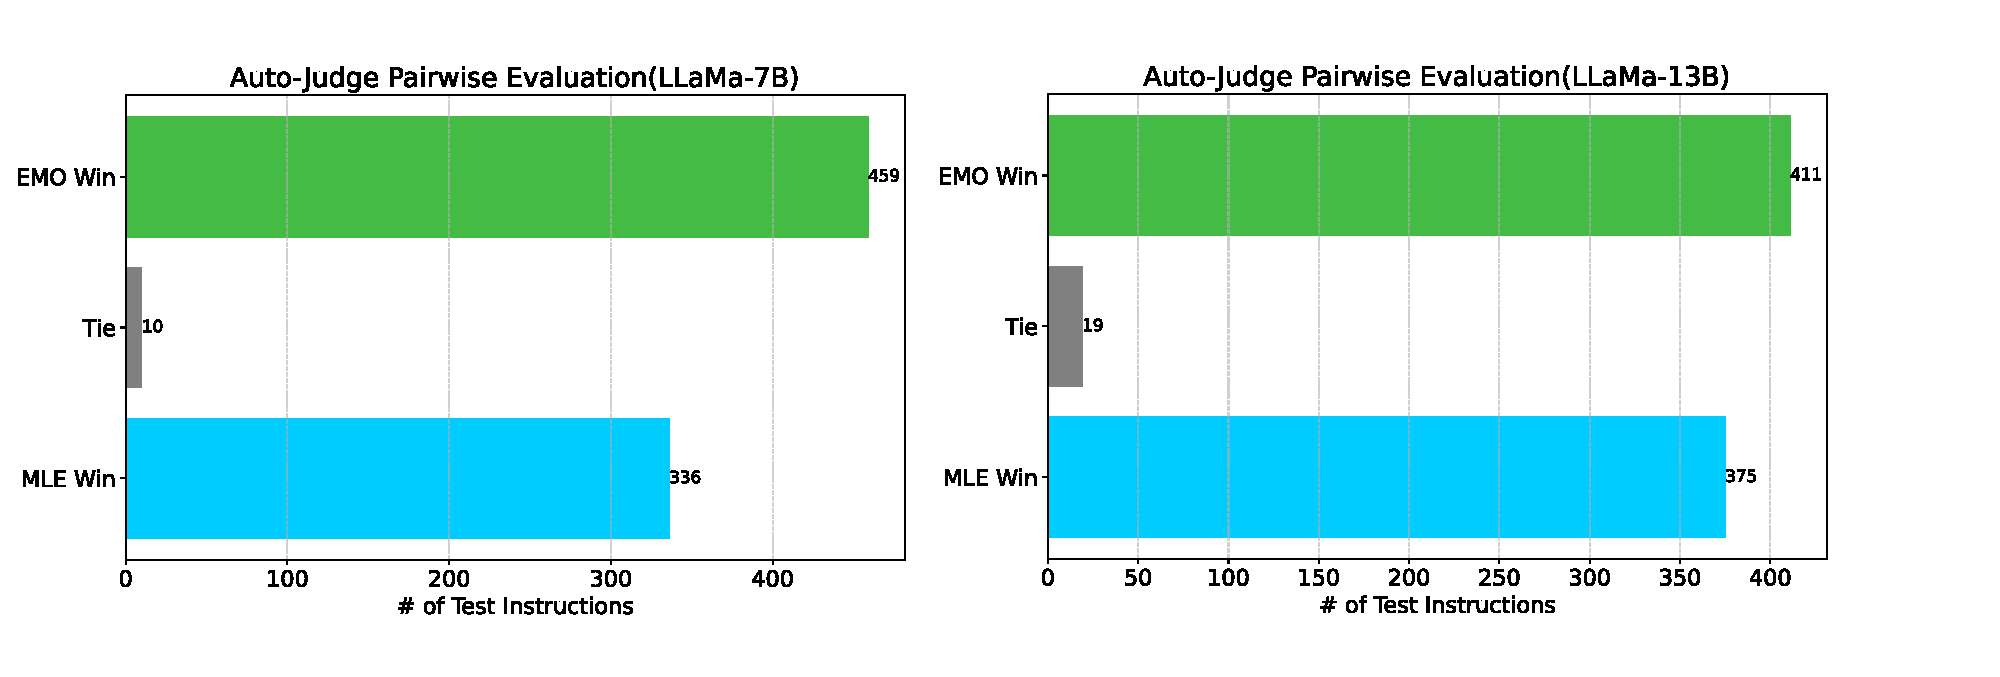
\includegraphics[width=0.99\textwidth]{./figures/auto-j-llama1.pdf}}
    \caption{Auto-J pairwise response comparison results of LLaMa-7B/13B fine-tuned with MLE and EMO on 805 test instructions from AlpacaEval.}
    \label{fig:autoj}
\end{figure}
\begin{figure}[h]
    \centering
    \scalebox{1.0}{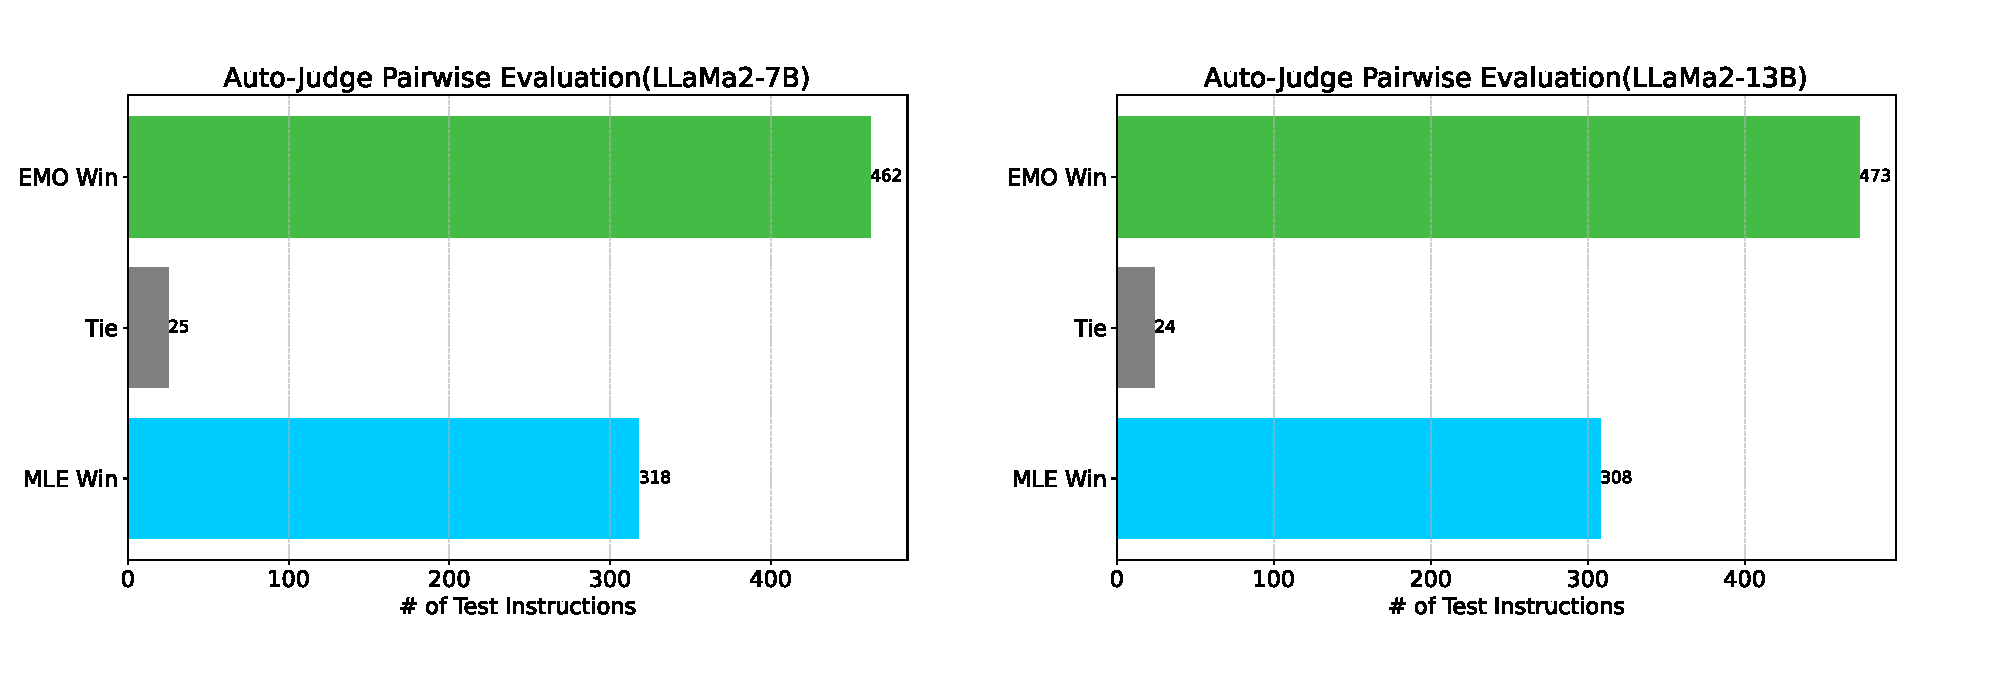
\includegraphics[width=0.99\textwidth]{./figures/auto-j-llama2.pdf}}
    \caption{Auto-J pairwise response comparison results of LLaMa2-7B/13B fine-tuned with MLE and EMO on 805 test instructions from AlpacaEval.}
    \label{fig:autoj-llama2}
\end{figure}

\begin{figure}[h]
    \centering
    \scalebox{1.0}{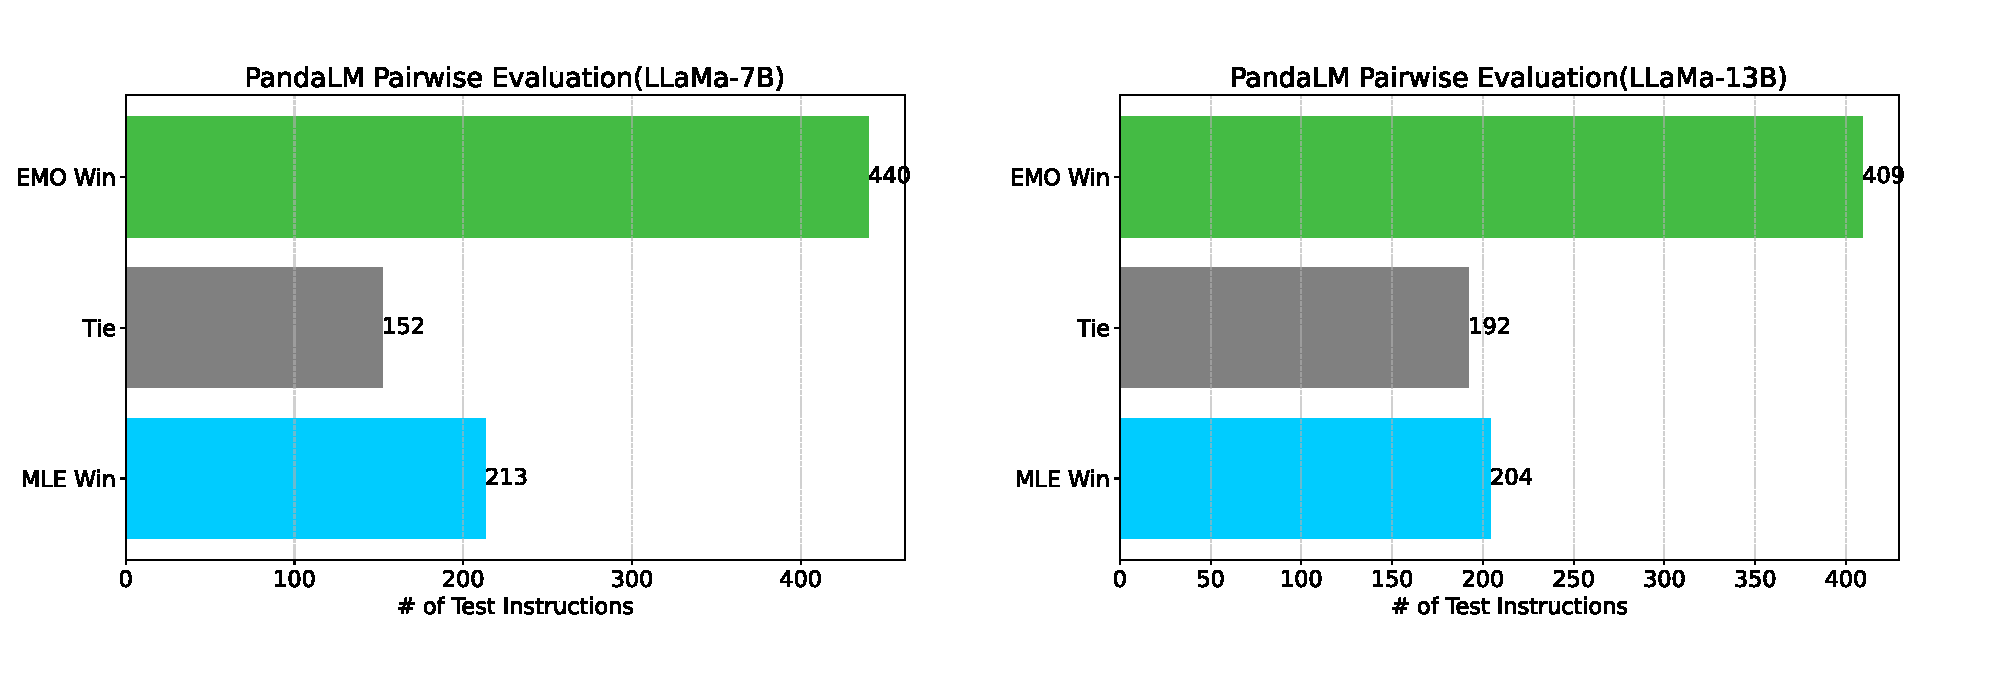
\includegraphics[width=0.99\textwidth]{./figures/pandalm_llama1.pdf}}
    \caption{PandaLM pairwise response comparison results of LLaMa-7B/13B fine-tuned with MLE and EMO on 805 test instructions from AlpacaEval.}
    \label{fig:pandalm_llama1}
\end{figure}
\begin{figure}[h]
    \centering
    \scalebox{1.0}{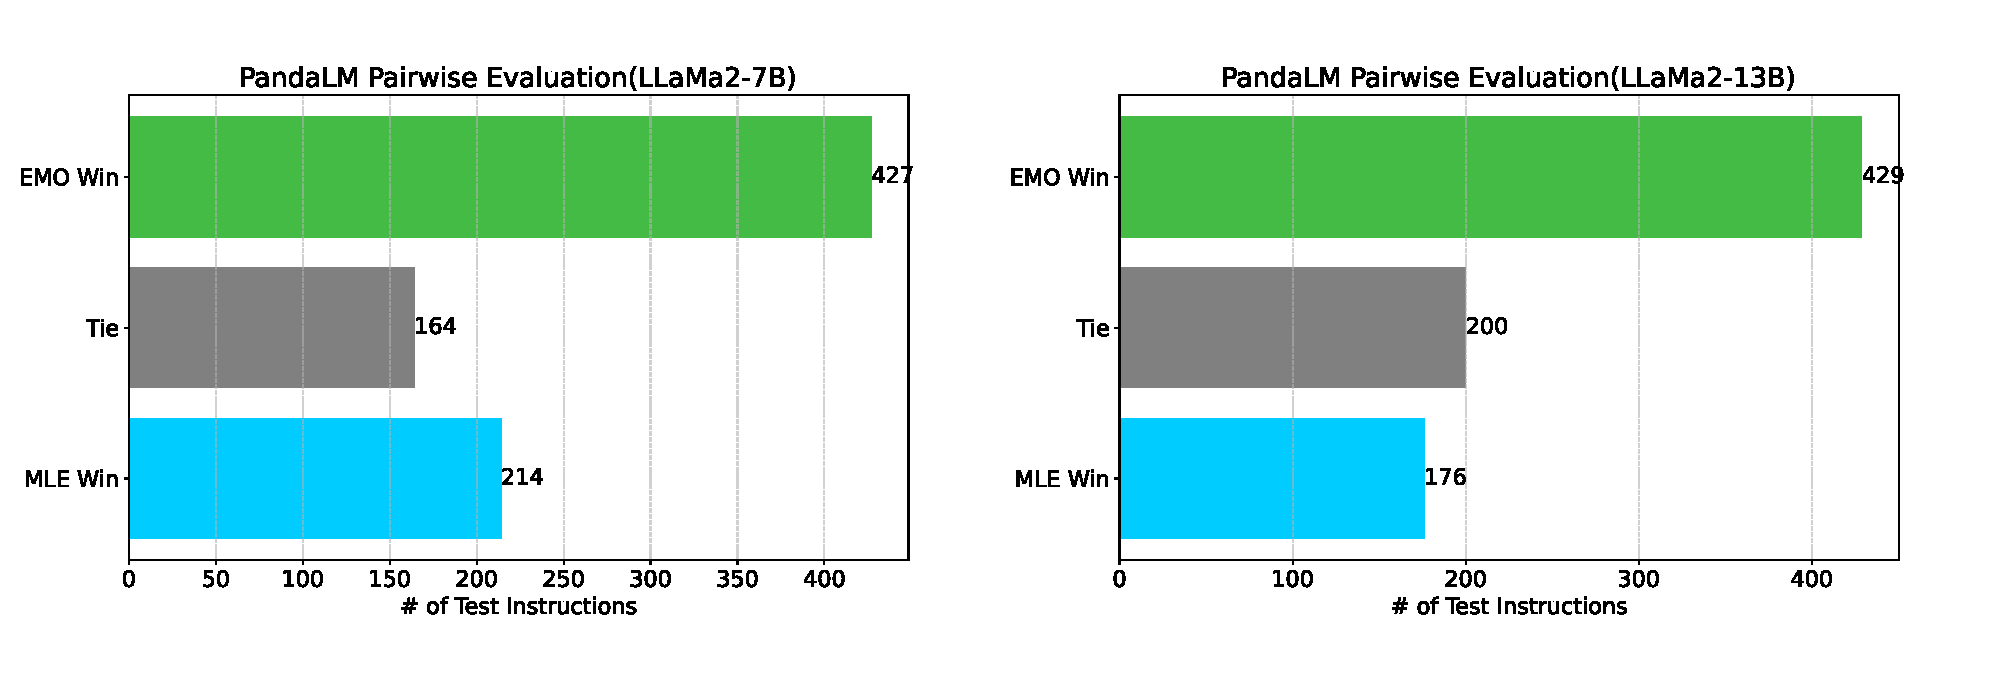
\includegraphics[width=0.99\textwidth]{./figures/pandalm_llama2.pdf}}
    \caption{PandaLM pairwise response comparison results of LLaMa2-7B/13B fine-tuned with MLE and EMO on 805 test instructions from AlpacaEval.}
    \label{fig:pandalm_llama2}
\end{figure}
